\chapter{การติดตั้งเครื่องมือที่ใช้พัฒนาโปรแกรม}
การติดตั้งเครื่องมือที่ใช้ในการพัฒนาแอปพลิเคชันระบบกองทุนเงินให้กู้ยืมเพื่อการศึกษา คณะวิทยาศาสตร์ มหาวิทยาลัยอุบลราชธานี มีโปรแกรมที่จำเป็นในการพัฒนาระบบดังต่อไปนี้
\begin{itemize}
	\item การติดตั้ง Android Studio
	\item การติดตั้ง Tensorflow Lite
\end{itemize}

\section{การติดตั้ง Android Studio}
\begin{enumerate}
	\item สามารถดาวน์โหลด Android Studio installer package ได้ที่ https://developer.android.com/studio/ ดังแสดงในรูปที่ \ref{Fig:android1}
	\begin{figure}[H]
		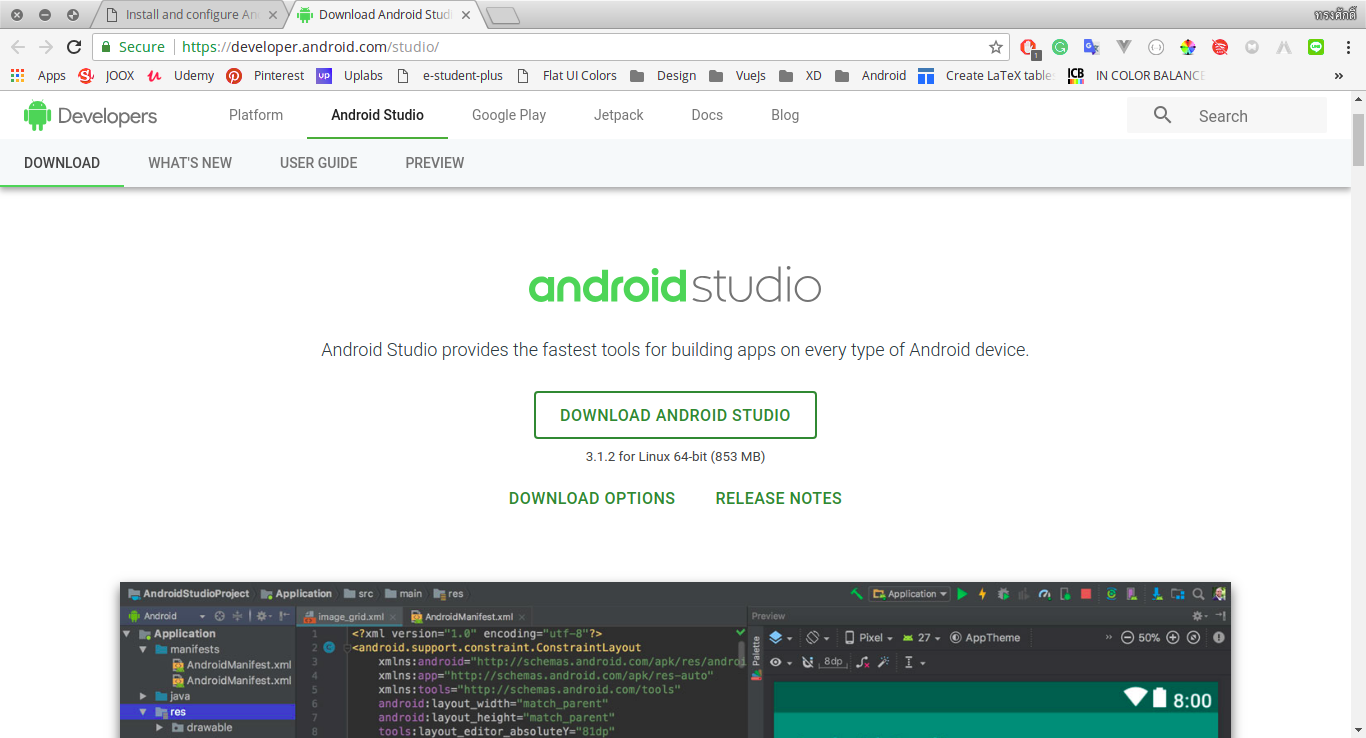
\includegraphics[width=\columnwidth]{Figures/prepareation/android1}
		\caption{หน้าเว็บดาวน์โหลด Android Studio}
		\label{Fig:android1}
	\end{figure}
	
	\item  แสดงหน้าต่างต้อนรับของ  Android Studio ทำการกด Next เพื่อเริ่มกระบวนการติดตั้ง ดังแสดงในรูปที่ \ref{Fig:android2}
	\begin{figure}[H]
		\centering
		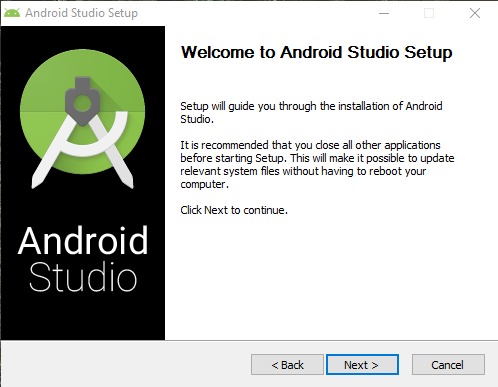
\includegraphics[width=0.7\columnwidth]{Figures/prepareation/android2}
		\caption{หน้าต่างต้อนรับของ  Android Studio}
		\label{Fig:android2}
	\end{figure}
	
	\item  แสดงหน้าต่างข้อตกลงการใช้งาน Android Studio ทำการกด  I Agree ดังแสดงในรูปที่ \ref{Fig:android4}
	\begin{figure}[H]
		\centering
		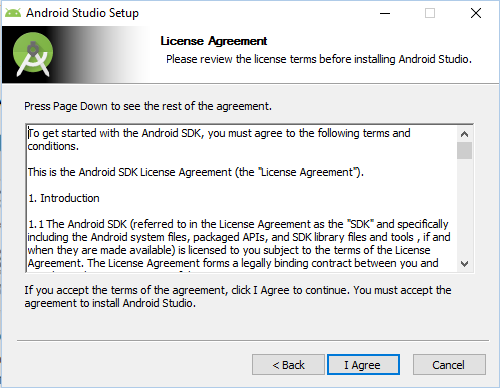
\includegraphics[width=0.7\columnwidth]{Figures/prepareation/android4}
		\caption{หน้าต่างข้อตกลงการใช้งาน  Android Studio}
		\label{Fig:android4}
	\end{figure}
	
	\item  แสดงหน้าต่างที่จัดเก็บไฟล์ต่างๆ ของ Android Studio ทำการกด Next ดังแสดงในรูปที่ \ref{Fig:android5}
	\begin{figure}[H]
		\centering
		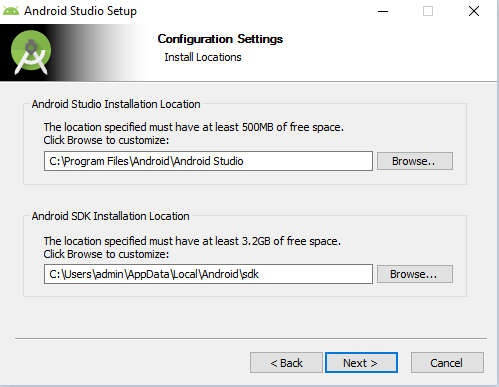
\includegraphics[width=0.7\columnwidth]{Figures/prepareation/android5}
		\caption{หน้าต่างที่จัดเก็บไฟล์ต่างๆ ของ  Android Studio}
		\label{Fig:android5}
	\end{figure}
	
	\item  หน้าต่างเริ่มทำการติดตั้งทำการกด Install ดังแสดงในรูปที่ \ref{Fig:android6}
	\begin{figure}[H]
		\centering
		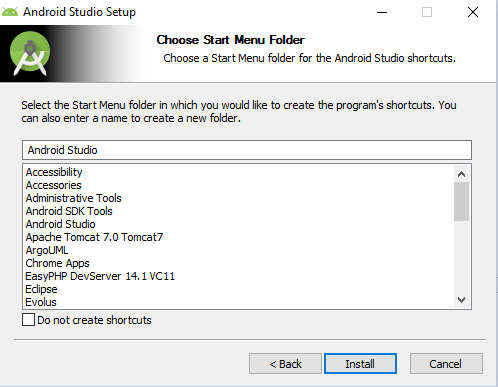
\includegraphics[width=0.7\columnwidth]{Figures/prepareation/android6}
		\caption{หน้าต่างที่จัดเก็บไฟล์ต่างๆ ของ  Android Studio}
		\label{Fig:android6}
	\end{figure}
	
	\item  หน้าต่างผลการติดตั้ง Android Studio ดังแสดงในรูปที่ \ref{Fig:android7}
	\begin{figure}[H]
		\centering
		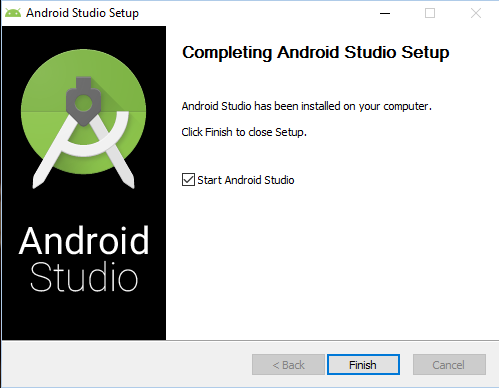
\includegraphics[width=0.7\columnwidth]{Figures/prepareation/android7}
		\caption{ หน้าต่างผลการติดตั้ง Android Studio}
		\label{Fig:android7}
	\end{figure}
	
\end{enumerate}

\newpage
\section{การติดตั้ง Python3.6}
	\begin{enumerate}
		\item การติดตั้ง Python3.6 สามารถดาวน์โหลดได้ที่ https://www.python.org/downloads/release/python-365/ ดังแสดงในภาพที่ \ref{Fig:py}
			\begin{figure}[H]
				\includegraphics[width=\columnwidth]{Figures/appendix1/py}
				\caption{หน้าเว็บดาวน์โหลด Python3.6}
				\label{Fig:py}
			\end{figure}
		\item เปิดไฟล์จะได้หน้าตาดังรูปที่ \ref{Fig:py2} จากนั้นกด Install now รอจนเสร็จ
			\begin{figure}[H]
				\includegraphics[width=\columnwidth]{Figures/appendix1/py2}
				\caption{การติดตั้ง Python3.6}
				\label{Fig:py2}
			\end{figure}
	\end{enumerate}
	
\newpage
\section{การติดตั้ง Tensorflow}
	โดยในการติดตั้งผ่าน pip สามารถเลือกได้ว่าจะให้ทำงานบน CPU อย่างเดียว หรือทำงานทั้งบน CPU และ GPU โดยมีคำสั่งดังนี้
	\begin{enumerate}
    	\item การติดตั้งสำหรับทำงานบน CPU  ดังแสดงในภาพที่ \ref{Fig:tensorCPU}
			\begin{figure}[H]
				{\setstretch{1.0}\begin{lstlisting}
pip3 install --upgrade tensorflow
				\end{lstlisting}}
				\caption{การติดตั้ง Tensorflow สำหรับทำงานบน CPU}
				\label{Fig:tensorCPU}
			\end{figure}

   		\item การติดตั้งสำหรับทำงานบน CPU และ GPU ดังแสดงในภาพที่ \ref{Fig:tensorGPU}
			\begin{figure}[H]
				{\setstretch{1.0}\begin{lstlisting}
pip3 install --upgrade tensorflow-gpu
				\end{lstlisting}}
				\caption{การติดตั้ง Tensorflow สำหรับทำงานบน CPU และ GPU}
				\label{Fig:tensorGPU}
			\end{figure}
	\end{enumerate}
